\documentclass[conference,a4paper]{IEEEtran}
\usepackage[T1]{fontenc}
\usepackage{amsmath}
\usepackage{graphicx}
\usepackage{booktabs}
\usepackage{cite}
\usepackage[hidelinks]{hyperref}
\usepackage{xurl}
% generated by code/make_macros.py -- do not edit
\makeatletter
\expandafter\def\csname res@altOneN\endcsname{18}
\expandafter\def\csname res@altOneP\endcsname{<0.001}
\expandafter\def\csname res@altOnePT\endcsname{<0.001}
\expandafter\def\csname res@altOnePos\endcsname{18}
\expandafter\def\csname res@altThreeN\endcsname{19}
\expandafter\def\csname res@altThreeP\endcsname{=0.36}
\expandafter\def\csname res@altThreePT\endcsname{0.36}
\expandafter\def\csname res@altThreePos\endcsname{12}
\expandafter\def\csname res@altTwoN\endcsname{13}
\expandafter\def\csname res@altTwoP\endcsname{=0.002}
\expandafter\def\csname res@altTwoPT\endcsname{0.002}
\expandafter\def\csname res@altTwoPos\endcsname{12}
\expandafter\def\csname res@cisoNlEarly\endcsname{20}
\expandafter\def\csname res@cisoNlLate\endcsname{21}
\expandafter\def\csname res@cisoRampEarly\endcsname{28}
\expandafter\def\csname res@cisoRampLate\endcsname{48}
\expandafter\def\csname res@dropped\endcsname{WALC}
\expandafter\def\csname res@ercoNlEarly\endcsname{17}
\expandafter\def\csname res@ercoNlLate\endcsname{21}
\expandafter\def\csname res@ercoRampEarly\endcsname{7}
\expandafter\def\csname res@ercoRampLate\endcsname{24}
\expandafter\def\csname res@errHighEarly\endcsname{3.0}
\expandafter\def\csname res@errHighLate\endcsname{3.7}
\expandafter\def\csname res@errHighN\endcsname{18}
\expandafter\def\csname res@errHighNNoCiso\endcsname{17}
\expandafter\def\csname res@errHighUp\endcsname{10}
\expandafter\def\csname res@errHighUpNoCiso\endcsname{9}
\expandafter\def\csname res@errLowEarly\endcsname{2.8}
\expandafter\def\csname res@errLowLate\endcsname{2.3}
\expandafter\def\csname res@errLowN\endcsname{24}
\expandafter\def\csname res@errLowUp\endcsname{9}
\expandafter\def\csname res@exclThreeN\endcsname{17}
\expandafter\def\csname res@exclThreeP\endcsname{=0.63}
\expandafter\def\csname res@exclThreePT\endcsname{0.63}
\expandafter\def\csname res@exclThreePos\endcsname{10}
\expandafter\def\csname res@hFourHolm\endcsname{=0.001}
\expandafter\def\csname res@hFourHolmT\endcsname{0.001}
\expandafter\def\csname res@hFourP\endcsname{<0.001}
\expandafter\def\csname res@hFourPT\endcsname{<0.001}
\expandafter\def\csname res@hOneHolm\endcsname{<0.001}
\expandafter\def\csname res@hOneHolmT\endcsname{<0.001}
\expandafter\def\csname res@hOneN\endcsname{17}
\expandafter\def\csname res@hOneP\endcsname{<0.001}
\expandafter\def\csname res@hOnePT\endcsname{<0.001}
\expandafter\def\csname res@hOnePos\endcsname{17}
\expandafter\def\csname res@hThreeHolm\endcsname{=0.48}
\expandafter\def\csname res@hThreeHolmT\endcsname{0.48}
\expandafter\def\csname res@hThreeN\endcsname{18}
\expandafter\def\csname res@hThreeNeg\endcsname{7}
\expandafter\def\csname res@hThreeP\endcsname{=0.48}
\expandafter\def\csname res@hThreePT\endcsname{0.48}
\expandafter\def\csname res@hThreePos\endcsname{11}
\expandafter\def\csname res@hTwoHolm\endcsname{=0.002}
\expandafter\def\csname res@hTwoHolmT\endcsname{0.002}
\expandafter\def\csname res@hTwoN\endcsname{14}
\expandafter\def\csname res@hTwoP\endcsname{<0.001}
\expandafter\def\csname res@hTwoPT\endcsname{<0.001}
\expandafter\def\csname res@hTwoPos\endcsname{13}
\expandafter\def\csname res@highApedlate\endcsname{3.0}
\expandafter\def\csname res@highApenllate\endcsname{3.8}
\expandafter\def\csname res@highHdearly\endcsname{17}
\expandafter\def\csname res@highHdlate\endcsname{17.5}
\expandafter\def\csname res@highHnlearly\endcsname{18}
\expandafter\def\csname res@highHnllate\endcsname{20}
\expandafter\def\csname res@levelBas\endcsname{FPC, PSCO, PSEI and WACM}
\expandafter\def\csname res@lowApedlate\endcsname{2.4}
\expandafter\def\csname res@lowApenllate\endcsname{2.3}
\expandafter\def\csname res@lowHdearly\endcsname{17.5}
\expandafter\def\csname res@lowHdlate\endcsname{18}
\expandafter\def\csname res@lowHnlearly\endcsname{18}
\expandafter\def\csname res@lowHnllate\endcsname{18}
\expandafter\def\csname res@lowShiftBas\endcsname{MISO, PJM, SC}
\expandafter\def\csname res@maxShift\endcsname{4}
\expandafter\def\csname res@maxShiftBa\endcsname{ERCO}
\expandafter\def\csname res@misoWind\endcsname{15}
\expandafter\def\csname res@nBas\endcsname{42}
\expandafter\def\csname res@nDaysMax\endcsname{244}
\expandafter\def\csname res@nDaysMin\endcsname{35}
\expandafter\def\csname res@nDropped\endcsname{1}
\expandafter\def\csname res@nHigh\endcsname{18}
\expandafter\def\csname res@nLow\endcsname{24}
\expandafter\def\csname res@nPrimary\endcsname{43}
\expandafter\def\csname res@paceNlEarly\endcsname{20}
\expandafter\def\csname res@paceNlLate\endcsname{21}
\expandafter\def\csname res@paceRampEarly\endcsname{9}
\expandafter\def\csname res@paceRampLate\endcsname{23}
\expandafter\def\csname res@rampEarly\endcsname{8.1}
\expandafter\def\csname res@rampLate\endcsname{15.3}
\expandafter\def\csname res@rampN\endcsname{18}
\expandafter\def\csname res@rampP\endcsname{<0.001}
\expandafter\def\csname res@rampPT\endcsname{<0.001}
\expandafter\def\csname res@rampPos\endcsname{16}
\expandafter\def\csname res@sepEarly\endcsname{11}
\expandafter\def\csname res@sepLate\endcsname{71}
\expandafter\def\csname res@sepN\endcsname{18}
\expandafter\def\csname res@sepP\endcsname{<0.001}
\expandafter\def\csname res@sepPT\endcsname{<0.001}
\expandafter\def\csname res@sepPos\endcsname{16}
\expandafter\def\csname res@shareMax\endcsname{32}
\expandafter\def\csname res@shareMaxBa\endcsname{PNM}
\expandafter\def\csname res@shareMin\endcsname{5}
\expandafter\def\csname res@shareMinBa\endcsname{SOCO}
\expandafter\def\csname res@shiftHigh\endcsname{1}
\expandafter\def\csname res@shiftLow\endcsname{0}
\expandafter\def\csname res@tenOneN\endcsname{9}
\expandafter\def\csname res@tenOneP\endcsname{=0.002}
\expandafter\def\csname res@tenOnePT\endcsname{0.002}
\expandafter\def\csname res@tenOnePos\endcsname{9}
\expandafter\def\csname res@tenThreeN\endcsname{10}
\expandafter\def\csname res@tenThreeP\endcsname{=0.75}
\expandafter\def\csname res@tenThreePT\endcsname{0.75}
\expandafter\def\csname res@tenThreePos\endcsname{6}
\expandafter\def\csname res@tenTwoN\endcsname{8}
\expandafter\def\csname res@tenTwoP\endcsname{=0.04}
\expandafter\def\csname res@tenTwoPT\endcsname{0.04}
\expandafter\def\csname res@tenTwoPos\endcsname{7}
\makeatother
\newcommand{\res}[1]{\ifcsname res@#1\endcsname\csname res@#1\endcsname\else\textbf{??#1??}\fi}

\newcommand{\repoURL}{https://github.com/Thanh-Van-2001/solar-peak-shift}

\begin{document}

\title{Utility Solar Is Moving the Net-Load Peak: Evidence from 42 U.S. Balancing Authorities, 2019--2026}

\author{\IEEEauthorblockN{Thanh Van Nguyen}
\IEEEauthorblockA{Tsinghua Shenzhen International Graduate School, Tsinghua University, Shenzhen, China\\
felicenguyen2001@gmail.com}}

\maketitle

\begin{abstract}
Utility-scale solar moves the hour at which net load (demand minus solar and wind) peaks into the evening, when dispatchable capacity, storage and imports must ramp up. Using hourly EIA-930 data for \res{nBas} U.S. balancing authorities (BAs) and a pre-specified analysis plan, we compare the summers of 2019--2020 with those of 2025--2026. In the \res{nHigh} BAs where utility solar supplied at least 5\% of 2025 demand, the median hour of the daily net-load peak moved later in all \res{hOneN} BAs with a change (Holm $p\res{hOneHolm}$), by a median of \res{perBaMedianShift} hour per BA (mean \res{perBaMeanShift}). The share of days with the net-load peak at hour ending 20 or later rose from \res{lateTwentyEarly}\% to \res{lateTwentyLate}\%, the gap to the demand peak widened in \res{hTwoPos} of \res{hTwoN} BAs, and the shift exceeded that of low-solar BAs (Holm $p\res{hFourHolm}$). The shift comes from solar rather than wind, and it survives month stratification, a comparison of 2019 with 2025 and the exclusion of BAs with suspect solar timestamps. The median three-hour ramp into the net-load peak grew \res{rampRatio}-fold per BA. The operators' published demand forecast was not measurably less accurate at the net-load peak hour than at the demand peak hour. Peak-oriented tariffs, demand response and forecast evaluation in solar-rich BAs should follow the net-load peak.
\end{abstract}

\begin{IEEEkeywords}
Solar energy, net load, peak demand, load forecasting, EIA-930.
\end{IEEEkeywords}

\section{Introduction}

As utility-scale solar grows, the residual demand that other resources must meet, the net load, falls at midday and peaks after sunset. California's ``duck curve'' made this familiar \cite{denholm2015duck}. A grid with high shares of variable generation has to be planned and operated around the evening ramp and the net-load peak rather than the demand peak, with storage and flexible converters taking a growing part \cite{kroposki2017renewable}. Forecasting work has followed, with net-load and solar forecasts for single systems \cite{wang2018netload,kaur2016benefits}.

How far the net-load peak has moved across the U.S. is less documented. Since July 2018, Form EIA-930 has reported hourly utility-scale solar and wind generation for the BAs of the Lower 48 that have such plants, next to demand and the BA's own day-ahead demand forecast \cite{eia930}. These files make a national comparison possible.

We use them, with an analysis plan committed to version control before any peak hour was computed, to ask three questions:
\begin{enumerate}
\item How far has the summer net-load peak moved between 2019--2020 and 2025--2026?
\item Has it separated from the demand peak?
\item Is the operators' demand forecast less accurate at the net-load peak?
\end{enumerate}

\section{Data and Methods}

\subsection{Data and sample}
We use hourly demand $D$, demand forecast $F$, utility solar $S$ and wind $W$ from the EIA-930 BALANCE files (November 2026 vintage), with the local date and hour. $S$ includes solar plants with and without integrated storage.

\emph{Screening.} Values of $D$ or $F$ that are non-positive or outside $[0.3,2]$ times the centred 168-hour median of demand are set to missing \cite{ruggles2020eia}, and negative $S$ or $W$ are set to zero. Net load is $\mathrm{NL}=D-S-W$.

\emph{Sample.} It starts from a fixed set of \res{nPrimary} BAs with median demand of at least 500~MW and near-complete demand and forecast series. The high-solar group consists of the \res{nHigh} BAs whose utility solar supplied at least 5\% of 2025 demand, from \res{shareMinBa} (\res{shareMin}\%) to \res{shareMaxBa} (\res{shareMax}\%). The low-solar group has the other \res{nLow}.

\emph{Periods and days.} The early period is June to September of 2019 and 2020; the late period is the same months of 2025 and 2026 (2026 to September). A day is used if all its hours have $D$, $F$ and NL. A BA needs at least 30 such days in each period; \res{dropped} fails this because of gaps in its solar and wind series. This leaves \res{nDaysMin} to \res{nDaysMax} days per BA and period.

\subsection{Quantities and hypotheses}
For each day, $h_D$ and $h_{\mathrm{NL}}$ are the hours (local hour ending) of the daily maxima of $D$ and NL. The evening ramp is the increase of NL over the three hours before its peak, in percent of the peak. Forecast accuracy is the absolute percentage error $100|F-D|/D$.

The plan fixed four hypotheses, with the BA as the unit:
\begin{itemize}
\item H1: in the high-solar group, the median $h_{\mathrm{NL}}$ is later in the late period in a majority of BAs.
\item H2: in the high-solar group, the gap between median $h_{\mathrm{NL}}$ and median $h_D$ grows.
\item H3: in the high-solar group in the late period, the forecast error at $h_{\mathrm{NL}}$ differs from that at $h_D$.
\item H4: the shift in median $h_{\mathrm{NL}}$ is larger in the high-solar group than in the low-solar group.
\end{itemize}
H1 and H2 use one-sided sign tests and H3 a two-sided one (ties dropped). H4 uses a one-sided Mann--Whitney test \cite{mann1947test}. Holm's procedure adjusts the four \cite{holm1979simple}. A pipeline check ran on CISO for 2019 and 2025 before the full run.

\emph{Amendments.} After the first run, five BAs that report no solar generation had dropped out of the low-solar group because their net load was undefined. We set a source a BA does not report, or that is below 1\% of its 2025 demand, to zero. No high-solar value changed, and H4 was supported before and after. After an internal review we added the exploratory checks of Section~\ref{sec:rob}. Both amendments are in the repository with all runs.

\section{Results}

Table~\ref{tab:hyp} summarises the four pre-specified tests and Table~\ref{tab:bas} the BA-level results.

\begin{table}[t]
\caption{Pre-specified hypotheses: BAs in the stated direction among those with a change, one- or two-sided $p$, Holm-adjusted $p$}
\label{tab:hyp}
\centering
\setlength{\tabcolsep}{3.5pt}
\begin{tabular}{llccc}
\toprule
 & Statement (high-solar group) & BAs & $p$ & Holm \\
\midrule
H1 & net-load peak later & \res{hOnePos}/\res{hOneN} & $\res{hOnePT}$ & $\res{hOneHolmT}$ \\
H2 & net-load minus demand peak grows & \res{hTwoPos}/\res{hTwoN} & $\res{hTwoPT}$ & $\res{hTwoHolmT}$ \\
H3 & error at net-load vs demand peak & \res{hThreePos}/\res{hThreeN} & $\res{hThreePT}$ & $\res{hThreeHolmT}$ \\
H4 & shift larger than low-solar$^\dagger$ & \res{nHigh} vs \res{nLow} & $\res{hFourPT}$ & $\res{hFourHolmT}$ \\
\bottomrule
\multicolumn{5}{l}{\footnotesize $^\dagger$Mann--Whitney $U=\res{hFourU}$.}
\end{tabular}
\end{table}

\begin{table}[t]
\caption{High-solar BAs: 2025 utility solar share, median hour (ending) of the summer net-load and demand peaks, and median three-hour evening ramp (\% of peak) in 2019--2020 $\to$ 2025--2026; late-period forecast error (\%) at the net-load / demand peak hour. $^\ddagger$Solar timestamps suspect (Section~\ref{sec:rob}); FPC and PSCO forecasts have large level gaps.}
\label{tab:bas}
\centering
\setlength{\tabcolsep}{4pt}
\begin{tabular}{lrcccc}
\toprule
BA & Solar \% & NL peak & Demand peak & Ramp & Error NL / D \\
\midrule
\csname @@input\endcsname tab_bas.tex
\bottomrule
\end{tabular}
\end{table}

\subsection{The net-load peak moved into the evening}
H1 was supported. In all \res{hOneN} high-solar BAs whose median $h_{\mathrm{NL}}$ changed, it moved later ($p\res{hOneP}$, Holm $p\res{hOneHolm}$). The per-BA shift had a median of \res{perBaMedianShift} hour and a mean of \res{perBaMeanShift} hours. The largest was \res{maxShift} hours, in \res{maxShiftBa}, and LDWP did not move. The group median moved from hour ending \res{highHnlearly} to \res{highHnllate}. Measured by the mean peak hour, the median BA's peak moved \res{meanShift} hours later (bootstrap 95\% interval over BAs \res{meanShiftLo} to \res{meanShiftHi}). The share of days with the net-load peak at hour ending 20 or later rose from \res{lateTwentyEarly}\% to \res{lateTwentyLate}\% (higher in \res{lateTwentyPos} of \res{lateTwentyN} BAs).

H4 was supported (Fig.~\ref{fig:shift}): the median shift was \res{shiftHigh} hour in the high-solar group and \res{shiftLow} in the low-solar group ($p\res{hFourP}$, Holm $p\res{hFourHolm}$). Across all \res{nBas} BAs the shift rose with solar share (Spearman $\rho=\res{rhoAll}$, $p\res{rhoAllP}$). Within the low-solar group it did not ($\rho=\res{rhoLow}$), although \res{lowShiftBas} shifted by two hours or more.

\begin{figure}[t]
\centering
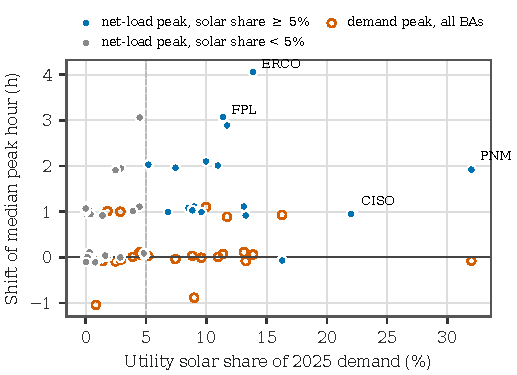
\includegraphics[width=\columnwidth]{fig_shift.pdf}
\caption{Change between the summers of 2019--2020 and 2025--2026 in the median hour of the daily net-load peak (filled) and demand peak (open), against the 2025 utility solar share (BAs reporting no solar at 0). Points are jittered vertically by up to 0.12 hours. Dashed line: the 5\% threshold.}
\label{fig:shift}
\end{figure}

\subsection{It separated from the demand peak}
H2 was supported: the gap between the net-load and demand peaks grew in \res{hTwoPos} of \res{hTwoN} high-solar BAs with a change ($p\res{hTwoP}$, Holm $p\res{hTwoHolm}$). The median demand peak barely moved, from \res{highHdearly} to \res{highHdlate}. Rooftop solar, which lowers reported demand at midday, would push the demand peak later too, so this test is conservative.

The secondary analyses show the consequences (Fig.~\ref{fig:cases}):
\begin{itemize}
\item The share of days with the net-load peak at least two hours after the demand peak rose from \res{sepEarly}\% to \res{sepLate}\% (group medians; higher in \res{sepPos} of \res{sepN} BAs, $p\res{sepP}$). It exceeded one half in \res{sepMajLate} BAs, against \res{sepMajEarly} before.
\item The three-hour ramp into the net-load peak rose from \res{rampEarly}\% to \res{rampLate}\% of the peak in group medians, a median \res{rampRatio}-fold per BA (higher in \res{rampPos} of \res{rampN}, $p\res{rampP}$). It fell in \res{rampFell}.
\item In ERCOT the net-load peak moved from hour ending \res{ercoNlEarly} to \res{ercoNlLate}, and its ramp grew from \res{ercoRampEarly}\% to \res{ercoRampLate}\%.
\end{itemize}

\begin{figure*}[t]
\centering
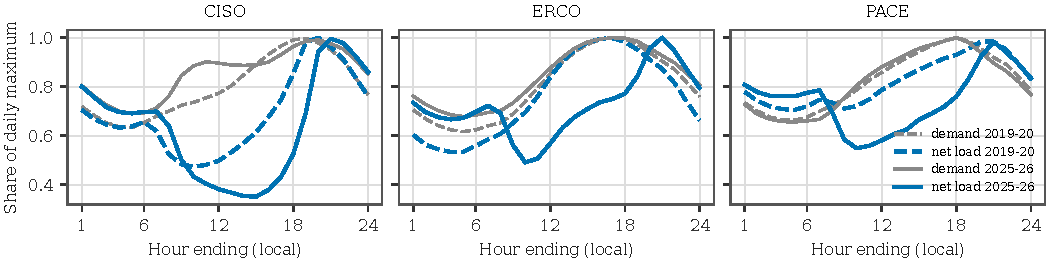
\includegraphics[width=\textwidth]{fig_cases.pdf}
\caption{Median summer profiles of demand (grey) and net load (blue), each divided by its daily maximum, in 2019--2020 (dashed) and 2025--2026 (solid). The three case BAs are fixed in the plan: CISO, ERCOT, and the largest solar share among other BAs above 5{,}000~MW (PACE). Profiles use all summer hours with demand and net load present, without the complete-day rule.}
\label{fig:cases}
\end{figure*}

\subsection{Forecast accuracy at the net-load peak}
H3 was not supported. In the late period, the operators' demand forecast was worse at each day's net-load peak hour than at its demand peak hour in \res{hThreePos} of \res{hThreeN} high-solar BAs ($p\res{hThreeP}$). The group medians were \res{highApenllate}\% and \res{highApedlate}\%.

Measuring at the realised peak hour selects on the outcome. In an exploratory check at fixed hours, each BA's late-period median $h_D$ and $h_{\mathrm{NL}}$, the error was worse at the net-load hour in \res{fixPos} of \res{fixN} BAs (median difference \res{fixDiff} points, Wilcoxon $p\res{fixW}$). With \res{hThreeN} BAs the test has little power, so the data show no difference, not equality.

The hour-of-day profiles add a caution (Fig.~\ref{fig:error}). The median error of high-solar BAs rose from \res{errHighEarly}\% to \res{errHighLate}\%, while that of low-solar BAs fell from \res{errLowEarly}\% to \res{errLowLate}\%. The rise was not uniform: it occurred in \res{errHighUp} of \res{errHighN} high-solar BAs, and in \res{errHighUpNoCiso} of \res{errHighNNoCiso} without CISO, whose forecast is offset by one hour from July 2022 to November 2025.

\begin{figure}[t]
\centering
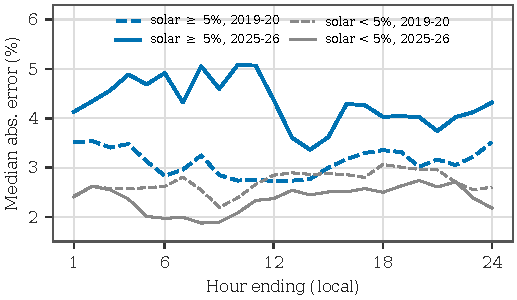
\includegraphics[width=\columnwidth]{fig_error.pdf}
\caption{Median absolute percentage error of the operators' day-ahead demand forecast by hour of day, median over BAs of each BA's median, for the high- and low-solar groups in 2019--2020 (dashed) and 2025--2026 (solid).}
\label{fig:error}
\end{figure}

\subsection{Robustness and attribution}\label{sec:rob}
The pre-specified variants agree. With three-year periods (2019--2021 against 2024--2026, which re-admits \res{dropped}):
\begin{itemize}
\item the net-load peak moved later in \res{altOnePos} of \res{altOneN} high-solar BAs;
\item the gap grew in \res{altTwoPos} of \res{altTwoN};
\item the error at the net-load peak was worse in \res{altThreePos} of \res{altThreeN} ($p\res{altThreeP}$).
\end{itemize}
With a 10\% solar threshold, the counts are \res{tenOnePos} of \res{tenOneN}, \res{tenTwoPos} of \res{tenTwoN} and \res{tenThreePos} of \res{tenThreeN}.

Exploratory checks added after an internal review address attribution and data quality:
\begin{itemize}
\item \emph{Solar, not wind.} With solar alone subtracted, H1 holds in \res{SolOnePos} of \res{SolOneN} BAs and H2 in \res{SolTwoPos} of \res{SolTwoN}. With wind alone, the counts are \res{WndOnePos} of \res{WndOneN} ($p\res{WndOneP}$) and \res{WndTwoPos} of \res{WndTwoN}.
\item \emph{Supply, not demand.} Swapping median profiles moves the net-load peak later by a median \res{supMed} hours when early demand meets late solar and wind (later in \res{supPos} of \res{supN} BAs). It moves it by \res{demMed} when late demand meets early generation.
\item \emph{Not storage.} Excluding solar plants with integrated storage leaves H1 and H2 unchanged (\res{NstOnePos} of \res{NstOneN}; \res{NstTwoPos} of \res{NstTwoN}).
\item \emph{Not the 2020 pandemic summer or the month mix.} 2019 against 2025 gives \res{YrOnePos} of \res{YrOneN} (median shift \res{yrShift} hours). Month-stratified shifts are later in \res{monthPos} of \res{monthN} BAs.
\item \emph{Not clocks.} Without the three BAs that do not observe daylight saving time, H1 holds in \res{nodstOnePos} of \res{nodstOneN}.
\item \emph{Not suspect solar timestamps.} In \res{tsBad} the solar series shows night-time output (up to \res{tsNightMax}\% of daily solar) or a drift of three hours or more in the hour of its daily maximum. Without them, H1 holds in \res{tsOnePos} of \res{tsOneN} and H2 in \res{tsTwoPos} of \res{tsTwoN}.
\item \emph{Not the forecast rule.} Dropping the requirement of a complete forecast changes nothing (\res{NoFOnePos} of \res{NoFOneN}).
\end{itemize}

\section{Discussion}

In the U.S. BAs with the most utility solar, the summer net-load peak has moved later by about an hour per BA in six years, and in ERCOT by four. It now falls at hour ending 20 or later on most days, often two hours or more after the demand peak, and the climb into it is steeper. Practices keyed to the demand peak are now aimed at a different hour from the net-load peak: coincident-peak tariffs, demand response windows and peak-oriented forecast evaluation. The steeper evening ramp is a requirement on flexible capacity, storage and the power electronics that connect them \cite{kroposki2017renewable}. This paper does not quantify those requirements.

The operators' published forecasts were not measurably worse at the net-load peak hour, but demand-forecast accuracy is not the target that matters there. Operators need net-load forecasts, which add solar and wind forecast errors that EIA-930 does not report \cite{wang2018netload,kaur2016benefits}.

\subsection*{Limitations}
\begin{itemize}
\item EIA-930 reports utility-scale solar only.
\item Peak hours are integers and two summers per period limit precision, which the mean-hour and share-of-days measures only partly offset.
\item Solar timestamps look suspect in three BAs. Results without them are reported, but other, smaller offsets cannot be ruled out.
\item The demand forecast is not a net-load forecast.
\item \res{dropped} is excluded from the primary analysis.
\end{itemize}

\section{Conclusion}
Across \res{nHigh} solar-rich U.S. balancing authorities, the summer net-load peak moved later by about an hour per BA between 2019--2020 and 2025--2026. It now lands at hour ending 20 or later on about two thirds of days and has separated from the demand peak. The shift is driven by solar and survives every check we ran. Tariffs, demand response and forecast evaluation should move with it.

\section*{Data and code availability}
The analysis plan with its commit history and amendments, the code and the result files are available at \url{\repoURL}. The EIA-930 data are public.

\section*{Acknowledgment}
The author used Claude Opus 5.5 (Anthropic; model identifier claude-opus-5-5) to help write analysis code and draft and edit the text. The author checked the code, the results and the text and takes full responsibility for the content.

\bibliographystyle{IEEEtran}
\bibliography{refs}

\end{document}
